\chapter{Simulation and Results}
\label{chap:5_Simulation_And_Results}
    
        %V1.0:
        % In this chapter, we present scenarios for validation and evaluation and experimental results. The scenarios cover different encounters between vessels for collision avoidance evaluation and for identification of our system's response and limitations we expose it to different wind speeds. Beyond that, we present the execution with and without \ac{ATC} for scientific control validation of the path planning algorithm. As done by several authors, \eg{} Larson \etal{} ~\cite{Larson2006Autonomous}, Naeem \etal{} ~\cite{Naeem2012COLREGS}, Campbell \etal{} ~\cite{Campbell2013Automatic}, Naus ~\cite{Naus2013Idea}, \etc{}, we evaluated 4 main encounter scenarios between two vessels: head-on, crossing from right, crossing from left and overtaking. Based on \cite{} we made a quantitative evaluation of our planning system measuring computational cost and minimum distance between vessels.
        
        %V2.0:
        % In this chapter, we present scenarios for validation (qualitative analysis) and evaluation (quantitative analysis) and experimental results. The scenarios cover different encounters between vessels for collision avoidance success evaluation and exposition to different environmental behaviors for identification of response capability and limitations of our system. Beyond that, we present the execution with and without \ac{ATC} for scientific control validation of our path planning algorithm.
        
        %V3.0:
        % In this chapter, we present the scenarios for validation (qualitative analysis) and evaluation (quantitative analysis) and experimental results. The scenarios cover different encounters between vessels for collision avoidance success evaluation and exposition to different environmental behaviors for identification of response capability and limitations of our system. Beyond that, we present the execution of our path planning algorithm with and without \ac{ATC}.
        
        %V4.0:
        % In this chapter, we present the scenarios for validation (qualitative analysis) and evaluation (quantitative analysis) of our approach, as well as the experimental results. The simulations cover different encounters scenarios between vessels for evaluation of collision avoidance success and exposition to different environmental behaviors for identification of limitations of our system.
        
        %V5.0:
        In this chapter, we present the scenarios for qualitative and quantitative evaluation of our approach, as well as the experimental results. The simulations cover different encounters scenarios between vessels for evaluation of collision avoidance success and exposition to different environmental behaviors for identification of limitations of our system.

    \section{Simulations Characterization}
    
    We run our simulations on \usvsim ~\cite{Paravisi2018Toward} simulator using the platform described in Table \ref{tab:simulation_platform_description}. 
    %Grammarlly: 100/100
    We developed 12 scenarios for evaluation the system focusing on being comparable with simulations presented in reference studies, \ie{} Agrawal \etal{} ~\cite{Agrawal2015COLREGS} and Huang \etal{} ~\cite{Huang2019Generalized}. Both studies were chosen for their quality ( \ie{} h-index) and similarity with our work. Agrawal \etal{} was chosen for being our problem-solving inspiration. Unfortunately, they do not present too much information about their system evaluation, so we based our tests and system evaluation on Huang \etal{} as they explicitly present their simulation scenarios characterization, results, and simulate a \ac{USV} similar in dimensions to ours.
    
    \taburowcolors[1] 1{tableLineOne .. tableLineTwo}
    \tabulinesep = ^3mm_2mm
    \everyrow{\tabucline[.4mm  white]{}}

    \begin{table}
        \caption{Simulation Platform Description}
        \centering
            \begin{tabu} to \textwidth { >{\bfseries}X[c, 0] X[c, 3]}
            \tableHeaderStyle
            Component & Specification \\
            Computer & Desktop Dell XPS 8700 \\
            Processor & Intel® Core™ i7-4770 CPU @ 3.40GHz × 8 \\
            Memory & \begin{tabular}[c]{@{}l@{}}Teikon PC3-12800u DDR3 1600 MHz 2GB x 2\\ Teikon PC3-12800u DDR3 1600 MHz 4GB x 2\end{tabular} \\
            Operating System & Ubuntu 16.04.6 LTS \\
            ROS Version & ROS Kinetic
            \end{tabu}  
        \label{tab:simulation_platform_description}
    \end{table}
    
        % Grammarlly: ?/100
    In our simulations, we use a differential boat - shown in Figure \ref{fig:diffboat} - with two thrusters, which enables it to rotate over its axis. This boat is modeled according to specifications of the Lutra Prop boat, acquired from Platypus ~\cite{PlatypusLLC}. Beyond the specifications shown in Table \ref{tab:diffboat_specs}, the Lutra boat we use in our simulation has in it bow, a laser rangefinder for environment scanning. We set the to be capable of detect objects up to 25 meters in a range of 360°.
%AMA acho q apresentacao do barco deva vir antes da apresentacao dos 4 cenarios. vc deve mencionar outras caracteristicas, como peso, sensores, a caracteristicas do laser.  
%DJ:    1- Boat: Done; 
%       2 - Outras caracteristicas: Done
    
    % \taburowcolors[1] 1{tableLineOne .. tableLineTwo}
    % \tabulinesep = ^3mm_2mm
    % \everyrow{\tabucline[.4mm  white]{}}
    % \begin{table}
    %     \caption{Lutra Prop parameters}
    %     \centering
    %         \begin{tabu} to 0.45\textwidth { >{\bfseries}X[c, 2] X[c, 2]}
    %         \tableHeaderStyle
    %         Parameter       & Value       \\
    %         Length          & 106 cm      \\
    %         Width           & 48 cm       \\
    %         Height          & 15 cm       \\
    %         % Hull Volume     & ~0.02 $m^3$ \\
    %         Weight          & 9.7 Kg      \\
    %         % Extra Payload   & 3 Kg        \\
    %         % Thruster Force  & 22.54 N     \\
    %         % Linear drag     & 11.33       \\
    %         Maximum speed   & 1.41 m/s    \\
    %         \end{tabu}  
    %     \label{tab:simulation_platform_description}
    % \end{table}
    
    \begin{minipage}{\textwidth}
        \begin{minipage}[b]{0.35\textwidth}
        \centering
        \begin{figure}[H]
            \centering
            \includegraphics[scale=0.75]{figs/Chap5/diffboat.png}
            % \caption{Simulated version of Lutra Prop boat}
            % \label{fig:diffboat}
        \end{figure}
        \captionof{figure}{Simulated version of Lutra Prop boat}
        \label{fig:diffboat}
        \end{minipage}
    %   \hfill
        \begin{minipage}[b]{0.5\textwidth}
        \centering
            \begin{tabular}{cc}
                \toprule
                    \textbf{Parameter}       & \textbf{Value}       \\
                \midrule
                    Length          & 106 cm      \\
                    Width           & 48 cm       \\
                    Height          & 15 cm       \\
                    Weight          & 9.7 Kg      \\
                    Maximum speed   & 1.41 m/s    \\ 
                \bottomrule
            \end{tabular}
        \captionof{table}{Lutra Prop parameters}
        \label{tab:diffboat_specs}
        \end{minipage}
    \end{minipage}
    
    \vskip 1cm
    
     We assembled the scenarios in a simulated version of the Dilúvio stream (see Figures \ref{fig:simulation_diluvio_googleLocation_roundedArea}, \ref{fig:simulation_diluvio_googleLocation2_1_roundedArea} and \ref{fig:simulation_diluvio_googleLocation2_2_roundedArea}), and as done by several authors, \eg{} Larson \etal{} ~\cite{Larson2006Autonomous}, Naeem \etal{} ~\cite{Naeem2012COLREGS}, Campbell \etal{} ~\cite{Campbell2013Automatic}, Naus ~\cite{Naus2013Idea}, \etc{}, we evaluated 4 main encounter scenarios between two vessels, head-on, crossing from right, crossing from Left, and overtaking. Figures \ref{fig:simulation_uwsim_headon_starting_pos}, \ref{fig:simulation_uwsim_crossingright_starting_pos}, \ref{fig:simulation_uwsim_crossingleft_starting_pos} and \ref{fig:simulation_uwsim_overtake_starting_pos} show the starting configuration of the evaluated scenarios, the respective configuration of each scenario is presented in Tables \ref{tab:simulation_scenarios_configuration_own_vessel} and \ref{tab:simulation_scenarios_configuration_encountering_vessel}.
    
    \begin{figure}[H]
        \centering
        \includegraphics[scale=0.3]{figs/Chap5/simulation_diluvio_googleLocation_roundedArea.png}
        \caption{Real-world location of the area we choose for evaluation of our system. This is a potential place for real-world trials of our system, once it is/has ... is near our laboratory, so we evaluate the behavior of our system on it. Google maps location (-30.047258°, -51.232660°), Av. Edvaldo Pereira Paiva, 1970 - Praia de Belas - Porto Alegre - RS - Brazil}
        \label{fig:simulation_diluvio_googleLocation_roundedArea}
    \end{figure}
    \todo{cite some characteristics of the region}
    
    \begin{figure}[H]
    \centering
        \begin{subfigure}[b]{0.55\textwidth}
            \centering
            \includegraphics[scale=0.1]{figs/Chap5/simulation_diluvio_googleLocation2_1_roundedArea.png}
            \caption{Real World}
            \label{fig:simulation_diluvio_googleLocation2_1_roundedArea}
        \end{subfigure}
        \begin{subfigure}[b]{0.42\textwidth}
            \centering
            \includegraphics[scale=0.1]{figs/Chap5/simulation_diluvio_googleLocation2_2_roundedArea.png}
            \caption{Real World Simulated}
            \label{fig:simulation_diluvio_googleLocation2_2_roundedArea}
        \end{subfigure}
    
    \caption{Real world region and its simulated version}
    \label{fig:simulation_diluvio_googleLocation2_roundedArea}
    \end{figure}
    
    % Grammarlly: 100/100
    Agrawal \etal ~\cite{Agrawal2015COLREGS} evaluate theirs A* approach in a 100mx100m grid with a resolution of 1:1, resulting in a search space of 10000 cells, we built our scenarios respecting the same proportionality. In all scenarios, our \ac{USV} plan in a 20mx20m grid with 1:0.2 resolution, resulting in a search space of 10000 cells, see Figure \ref{fig:rviz_local_costmap}. The choice of 20x20 dimension is related to real limitations of the range and reliability on laser sensors, the RPLIDAR A3 laser~\cite{RPLidarA3} model, for example, is reliably capable of detection in a 25 meters distance range.
    
    \begin{figure}[H]
    \centering
    
        \begin{subfigure}[b]{0.5\textwidth}
            \centering
            \includegraphics[width=\textwidth]{figs/Chap5/simulation_uwsim_headon_starting_pos.png}
            \caption{Head On}
            \label{fig:simulation_uwsim_headon_starting_pos}
        \end{subfigure}
        \begin{subfigure}[b]{0.45\textwidth}
            \centering
            \includegraphics[width=\textwidth]{figs/Chap5/simulation_uwsim_crossingright_starting_pos.png}
            \caption{Crossing from Right}
            \label{fig:simulation_uwsim_crossingright_starting_pos}
        \end{subfigure}
        
        \begin{subfigure}[b]{0.5\textwidth}
            \centering
            \includegraphics[width=\textwidth]{figs/Chap5/simulation_uwsim_crossingleft_starting_pos.png}
            \caption{Crossing from Left}
            \label{fig:simulation_uwsim_crossingleft_starting_pos}
        \end{subfigure}
        \begin{subfigure}[b]{0.45\textwidth}
            \centering
            \includegraphics[width=\textwidth]{figs/Chap5/simulation_uwsim_overtake_starting_pos.png}
            \caption{Overtaking}
            \label{fig:simulation_uwsim_overtake_starting_pos}
        \end{subfigure}
    
    \caption{Encounter scenarios for evaluation. Scenarios adopted from ~\cite{Huang2019Generalized}.}
    \label{fig:simulation_uwsim_encounters}
    \end{figure}

%AMA a figura dos barcos esta muito pequena. veja como fica na versao impressa. acho q vc vai ter q pelo menos desenhar uma flecha p indicar a direcao dos barcos.

    \begin{center}
        \savebox{\mytablebox}{\begin{tabular}{cccc}
        
        \toprule[3pt]
        \multicolumn{4}{c}{\textbf{Own Vessel}} \\
        \midrule
        \textbf{Encounter Type} & \textbf{Initial Pose (m, m, º)} & \textbf{Target Position} &  \textbf{Max. Speed (m/s)}\\
        \midrule
        Head On &  (450, 107.5, 0)  &   (480, 107.5)   &  0.4 \\
        Crossing Right &  (410, 105, 90)  &  (410, 133)   &  0.86  \\
        Crossing Left &  (410, 105, 90)  & (410, 133)   &  0.29  \\
        Overtaking &  (450, 107.5, 0)  &  (550, 107.5)   &  0.5 \\
        \bottomrule
        
        \end{tabular}}
        \settowidth{\mytablewidth}{\usebox{\mytablebox}}
        \begin{minipage}{\mytablewidth}
        \captionof{table}{Encounter Scenarios Configuration - Own Vessel}
        \label{tab:simulation_scenarios_configuration_own_vessel}
        \usebox{\mytablebox}
        \end{minipage}

    \end{center}
    
    \begin{center}
        \savebox{\mytablebox}{\begin{tabular}{cccc}
        
        \toprule[3pt]
        \multicolumn{4}{c}{\textbf{Encountering Vessel}} \\
        \midrule
        \textbf{Encounter Type} & \textbf{Initial Pose (m, m, º)} & \textbf{Target Position} & \textbf{Max. Speed (m/s)}\\
        \midrule
        Head On &  (450, 107.5, 0)  &   (480, 107.5)   &  0.4 \\
        Crossing Right &  (410, 105, 90)  &  (410, 133)   &  0.86  \\
        Crossing Left &  (410, 105, 90)  & (410, 133)   &  0.29  \\
        Overtaking &  (450, 107.5, 0)  &  (550, 107.5)   &  0.5 \\
        \bottomrule
        
        \end{tabular}}
        \settowidth{\mytablewidth}{\usebox{\mytablebox}}
        \begin{minipage}{\mytablewidth}
        \captionof{table}{Encounter Scenarios Configuration - Encountering Vessel}
        \label{tab:simulation_scenarios_configuration_encountering_vessel}
        \usebox{\mytablebox}
        \end{minipage}

    \end{center}

%AMA a apresentacao da tabela está realmente feia ! Latex tem formatos bem legais. Sugiro melhorar esse aspecto. Tb sugiro fortemente colocar na fig anterior o local do initial pose, destination, e trajetoria. Acho q deve trocar Waypoint por destination ou target position.
%DJ: Done
    
    \section{Experiments Results}
    
        % Grammarlly: 99/100
        % v1.0
        % We qualitatively evaluated the behavior of our method in two different configurations. In the first configuration, we compare the behavior of the system with and without ATC, and in the second configuration, we evaluate the behavior of our system with ATC under the influence of wind and without the influence of wind. We executed both scenarios for four types of possible encounters between two vessels. Results and their respective description are presented respectively in Figures \ref{fig:plots_ho}, \ref{fig:plots_cr}, \ref{fig:plots_cl} and \ref{fig:plots_ov}. For the quantitative evaluation of each scenario, we measured the computation time of every execution of our path planner, average sustained speed, and minimal distance maintained between the vessels, as well as we evaluated whether the collision avoidance was successful or not. In Table \ref{tab:results} we summarize the collected results.
        
        % Grammarlly: 99/100
        % v2.0
        We qualitatively evaluated the behavior of our method in two different configurations. In the first configuration, we compare the behavior of the system with and without ATC, and in the second configuration, we evaluate the behavior of our system with ATC under the influence of wind and without the influence of wind. We executed both scenarios for four types of possible encounters between two vessels. For the quantitative evaluation of each scenario, we measured the computation time of every execution of our path planner, average sustained speed, and minimal distance maintained between the vessels, as well as we evaluated whether the collision avoidance was successful or not. In Table \ref{tab:results} we summarize the collected results.
        
        Figure \ref{fig:plot_ho_w_vs_wo} presents, comparatively, the trajectory of two vessels in two executions of the same head-on scenario. In the "ATC case" execution, our system is fully functional, in the other "no ATC" execution, we removed the ability of the planning system to generate virtual obstacles, which is the core of the ATC method and partially responsible for the COLREGS-Compliant path planning. In both runs, in the time interval from t0 until just before t1 OV takes off in the north direction, this is due to an obstacle located from (450, 105) to (460, 105). Until t1 OV tends to distance itself from the static obstacle. At t1, for both executions of the scenario, EV becomes noticeable at the OV local cost map. From t1 OV react differently to each encounter. We observe that even with the existence of a static obstacle to the south in its proximity OV in ATC case decides to avoid the encounter with the other vessel moving to its starboard side, featuring a COLREGS-Compliant path. OV in "no ATC" influenced by the existence of an obstacle to the south and the encounter with EV, defines a not COLREGS-compliant path.
        
        % \begin{figure}[H]
        % \centering
        
        %     \begin{subfigure}[b]{0.45\textwidth}
        %         \centering
        %         \includegraphics[width=\textwidth]{figs/Chap5/plot_headOn_E.png}
        %         \caption{With \ac{ATC}}
        %         \label{fig:plot_headOn_E}
        %     \end{subfigure}
        %     \begin{subfigure}[b]{0.45\textwidth}
        %         \centering
        %         \includegraphics[width=\textwidth]{figs/Chap5/plot_noATC_headOn_E.png}
        %         \caption{Without \ac{ATC}}
        %         \label{fig:plot_noATC_headOn_E}
        %     \end{subfigure}
            
        %     \begin{subfigure}[b]{0.45\textwidth}
        %         \centering
        %         \includegraphics[width=\textwidth]{figs/Chap5/plot_headOn_Wind_E.png}
        %         \caption{With \ac{ATC} and Wind}
        %         \label{fig:plot_headOn_Wind_E}
        %     \end{subfigure}
        %     % \begin{subfigure}[b]{0.45\textwidth}
        %     %     \centering
        %     %     \includegraphics[width=\textwidth]{figs/Chap5/plot_Overtaking_Wind_BAD_E.png}
        %     %     \caption{\ac{ATC} and Bad Wind}
        %     %     \label{fig:plot_headOn_Wind__BAD_E}
        %     % \end{subfigure}
        
        % \caption{DESCRIÇÂO DOS GRAFICOS AQUI: }
        % \label{fig:headOn_E}
        % \end{figure}
%AMA a legenda dass trajetorias esta ilegivel. ou vc aumenta ate ficar legivel ou remove dali. se remover, vc pode descrever o significado das cores na legenda.
%AMA do jeito q está, nao eh facil comparar um grafico c o outro. seria MUITO melhor se vc conseguir colocar dois plots juntos. por exemplo, with ATC e wo/ ATC. with ATC e with ATC + wind. Nao junta os 3 pois acho q vai poluir demais.
% AMA a legenda dos eixos tb nao deve estar legivel p impressao. aumente o texto dos nros.
%AMA o ponto vermelho eh o ponto inicial ou final. deixar isso claro na legenda
%AMA qnd tiver vento, anota na figura a dirececao e velocidade tb.

        \begin{figure}[H]
            \centering
            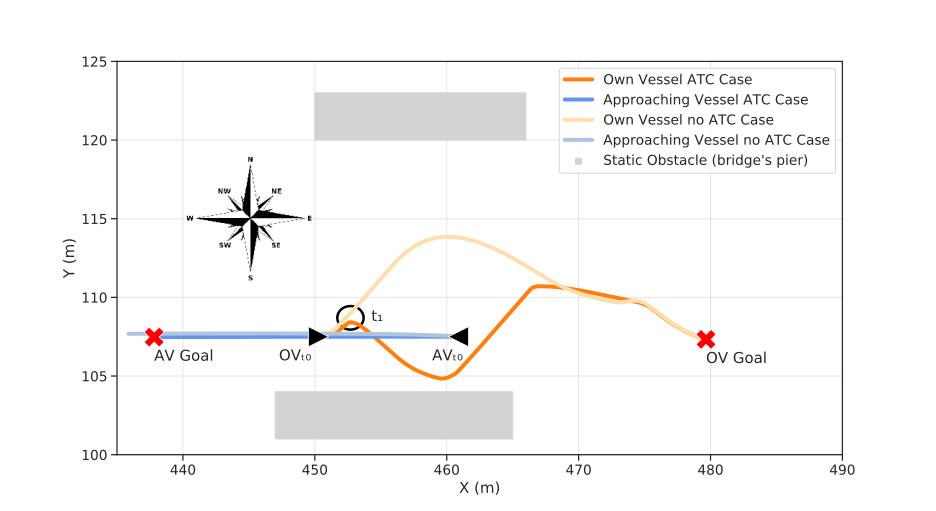
\includegraphics[scale=0.5]{figs/Chap5/plot_ho_w_vs_wo.png}
            \caption{Path planning comparison between ATC case versus no ATC in a head-on encounter.}
            \label{fig:plot_ho_w_vs_wo}
        \end{figure}
        
        Figure \ref{fig:plot_ho_w_vs_wo_CT} shows the computational time measured in seconds in the time series. As we can see, both ATC case and no ATC have similar computational cost curves. This is due to the fact that the computational cost of our path planning method is related to our A* implementation. The ATC method alone has low computational consumption since it cost in the worst case in filling an area lxm, with l = OV size and m = costmap.greaterDimension () / 2 that is O (n²);
        
        \begin{figure}[H]
            \centering
            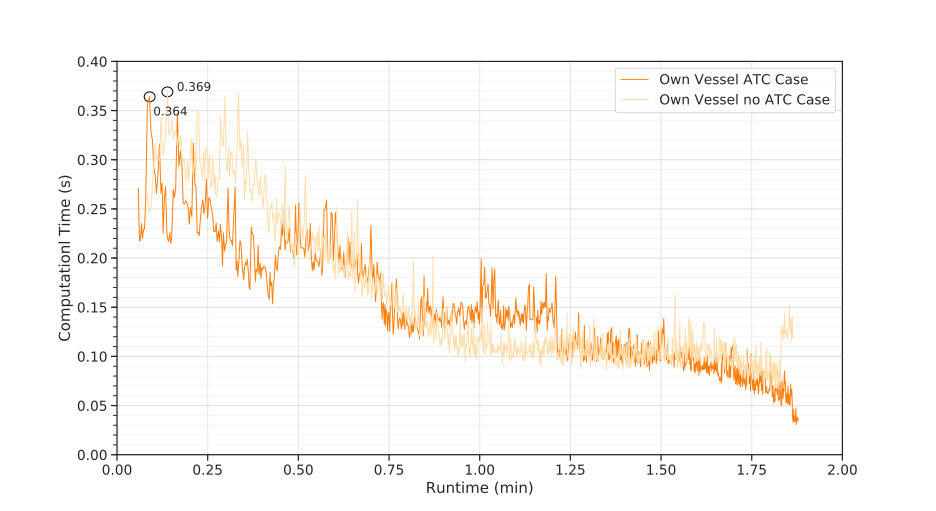
\includegraphics[width=\textwidth]{figs/Chap5/plot_ho_w_vs_wo_CT.png}
            \caption{Computational time comparison between ATC case versus no ATC in a head-on encounter}
            \label{fig:plot_ho_w_vs_wo_CT}
        \end{figure}
        
        % \begin{figure}[H]
        % \centering
        
        %     \begin{subfigure}[b]{0.45\textwidth}
        %         \centering
        %         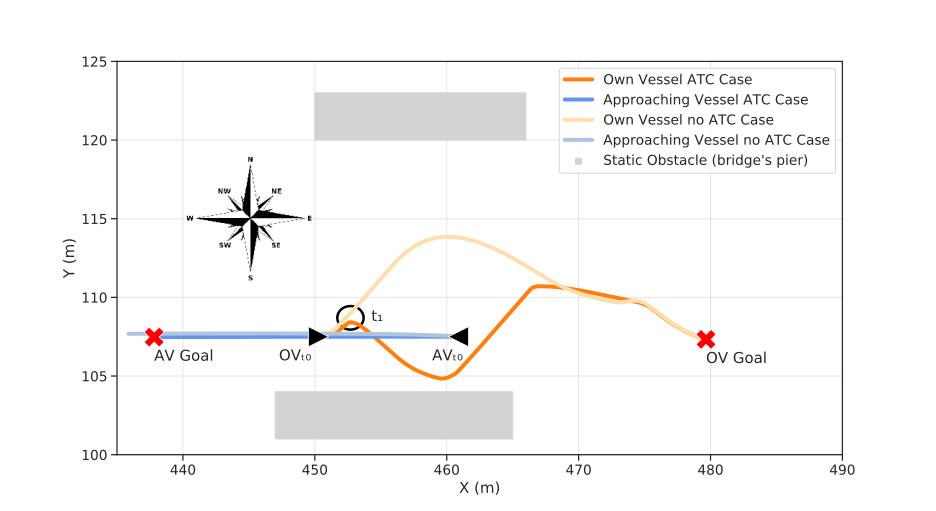
\includegraphics[width=\textwidth]{figs/Chap5/plot_ho_w_vs_wo.png}
        %         \caption{Route}
        %         \label{fig:plot_ho_w_vs_wo}
        %     \end{subfigure}
        %     \begin{subfigure}[b]{0.45\textwidth}
        %         \centering
        %         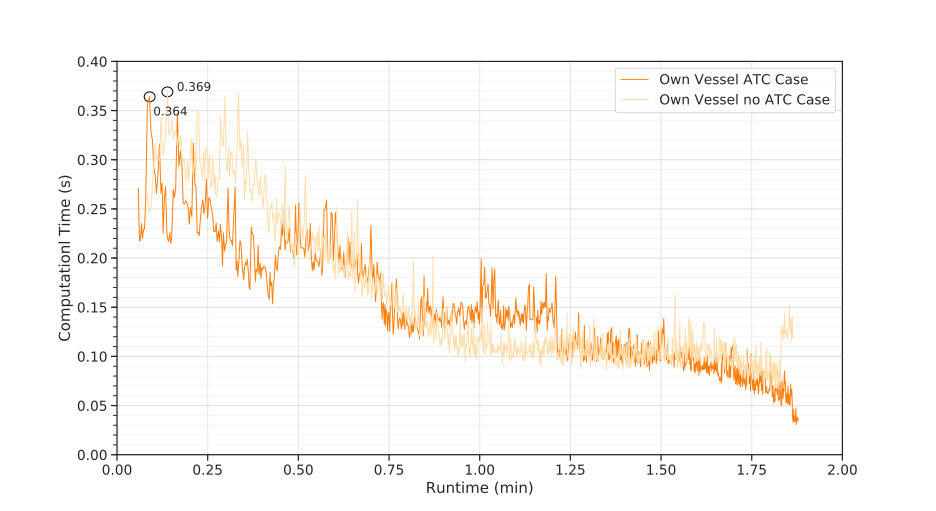
\includegraphics[width=\textwidth]{figs/Chap5/plot_ho_w_vs_wo_CT.png}
        %         \caption{Computation Time}
        %         \label{fig:plot_ho_w_vs_wo_CT}
        %     \end{subfigure}
        
        % \caption{Head On Encounter Scenario with and without ATC. \ref{fig:plot_ho_w_vs_wo} description aqui. \ref{fig:plot_ho_w_vs_wo_CT} description aqui}
        % \label{fig:plots_ho_w_vs_wo}
        % \end{figure}
        
        % \begin{figure}[H]
        % \centering
            
        %     \begin{subfigure}[b]{0.45\textwidth}
        %         \centering
        %         \includegraphics[width=\textwidth]{figs/Chap5/plot_ho_w_vs_wind.png}
        %         \caption{Route}
        %         \label{fig:plot_ho_w_vs_wind}
        %     \end{subfigure}
        %     \begin{subfigure}[b]{0.45\textwidth}
        %         \centering
        %         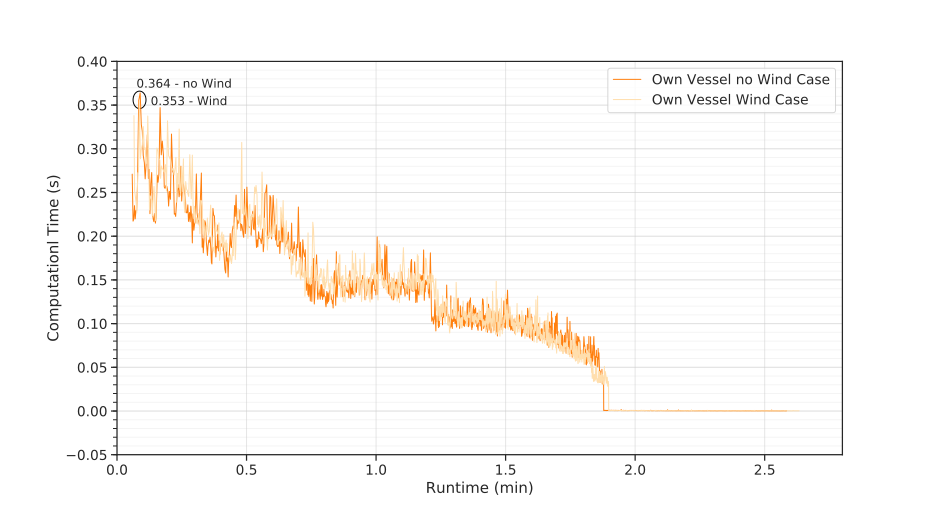
\includegraphics[width=\textwidth]{figs/Chap5/plot_ho_w_vs_wind_CT.png}
        %         \caption{Computation Time}
        %         \label{fig:plot_ho_w_vs_wind_CT}
        %     \end{subfigure}
        
        % \caption{Head On Encounter Scenario with ATC, with and without wind. \ref{fig:plot_ho_w_vs_wind} description aqui. \ref{fig:plot_ho_w_vs_wind_CT} description aqui}
        % \label{fig:plots_ho_w_vs_wind}
        % \end{figure}
        
        %%%%%%%%%%%%%%%%%%%%%%%%%%%%%%%%%%%%%%
        %% Head-On w vs wo ATC. w vs wo Wind
        %%%%%%%%%%%%%%%%%%%%%%%%%%%%%%%%%%%%%%
        \begin{figure}[H]
        \centering
        
            \begin{subfigure}[b]{0.49\textwidth}
                \centering
                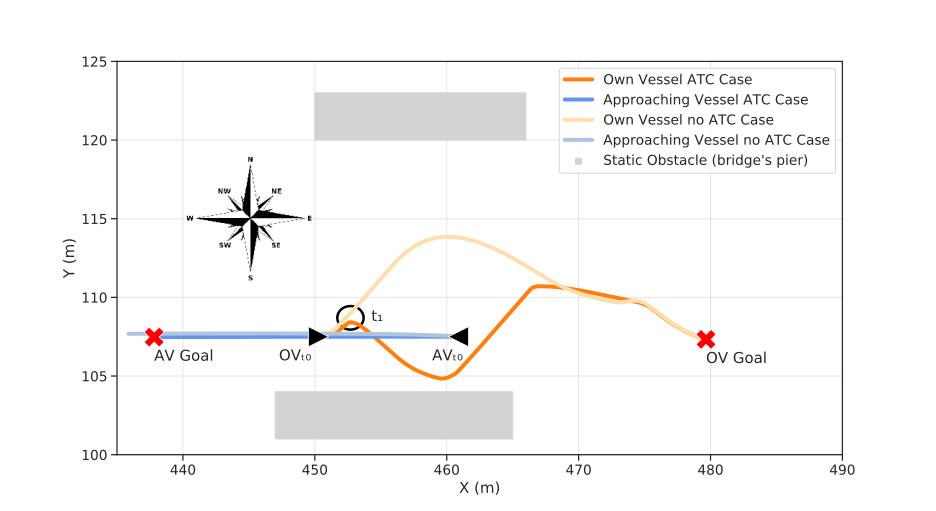
\includegraphics[width=\textwidth]{figs/Chap5/plot_ho_w_vs_wo.png}
                \caption{}
                \label{fig:plot_ho_w_vs_wo}
            \end{subfigure}
            \begin{subfigure}[b]{0.49\textwidth}
                \centering
                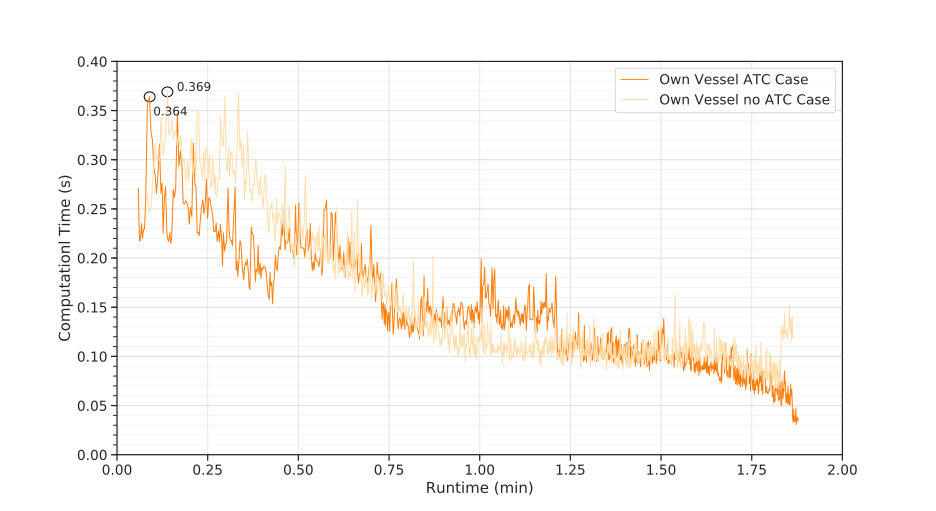
\includegraphics[width=\textwidth]{figs/Chap5/plot_ho_w_vs_wo_CT.png}
                \caption{}
                \label{fig:plot_ho_w_vs_wo_CT}
            \end{subfigure}
            
            \begin{subfigure}[b]{0.49\textwidth}
                \centering
                \includegraphics[width=\textwidth]{figs/Chap5/plot_ho_w_vs_wind.png}
                \caption{}
                \label{fig:plot_ho_w_vs_wind}
            \end{subfigure}
            \begin{subfigure}[b]{0.49\textwidth}
                \centering
                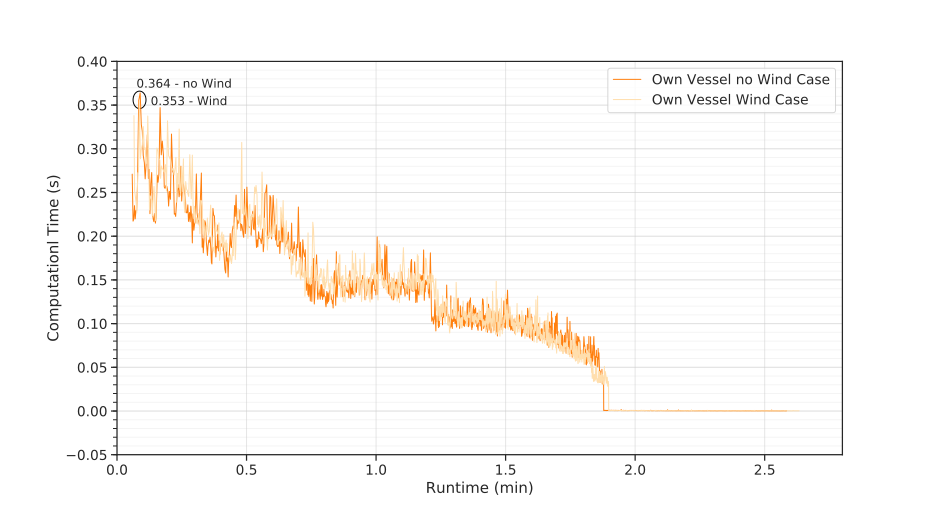
\includegraphics[width=\textwidth]{figs/Chap5/plot_ho_w_vs_wind_CT.png}
                \caption{}
                \label{fig:plot_ho_w_vs_wind_CT}
            \end{subfigure}
        
        \caption{Head On Encounter Scenario with ATC, with and without wind. \ref{fig:plot_ho_w_vs_wo} and \ref{fig:plot_ho_w_vs_wo_CT}  description aqui. \ref{fig:plot_ho_w_vs_wind} and \ref{fig:plot_ho_w_vs_wind_CT} description aqui}
        \label{fig:plots_ho}
        \end{figure}
        
        %%%%%%%%%%%%%%%%%%%%%%%%%%%%%%%%%%%%%%
        %% Crossing Right w vs wo ATC. w vs wo Wind
        %%%%%%%%%%%%%%%%%%%%%%%%%%%%%%%%%%%%%%
        \begin{figure}[H]
        \centering
        
            \begin{subfigure}[b]{0.45\textwidth}
                \centering
                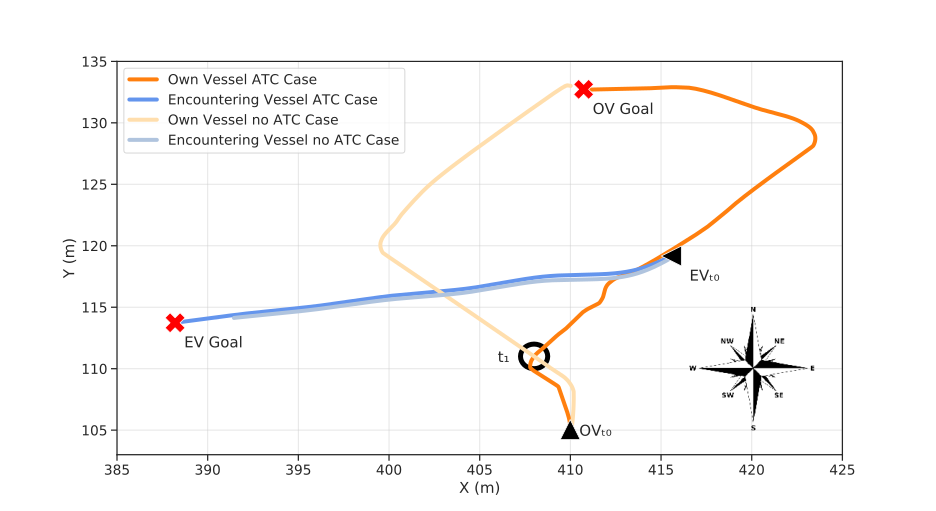
\includegraphics[width=\textwidth]{figs/Chap5/plot_cr_w_vs_wo.png}
                \caption{Route}
                \label{fig:plot_cr_w_vs_wo}
            \end{subfigure}
            \begin{subfigure}[b]{0.45\textwidth}
                \centering
                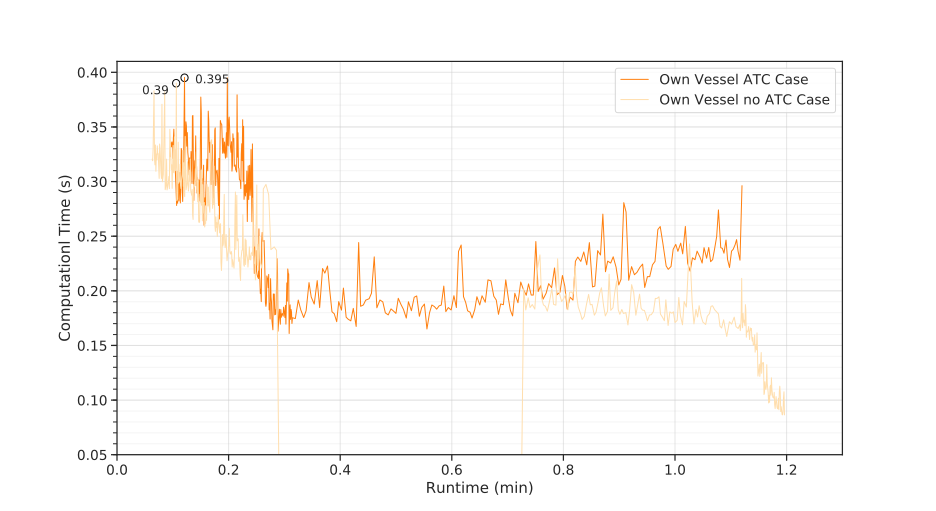
\includegraphics[width=\textwidth]{figs/Chap5/plot_cr_w_vs_wo_CT.png}
                \caption{Computation Time}
                \label{fig:plot_cr_w_vs_wo_CT}
            \end{subfigure}
            
            \begin{subfigure}[b]{0.45\textwidth}
                \centering
                \includegraphics[width=\textwidth]{figs/Chap5/plot_cr_w_vs_wind.png}
                \caption{Route}
                \label{fig:plot_cr_w_vs_wind}
            \end{subfigure}
            \begin{subfigure}[b]{0.45\textwidth}
                \centering
                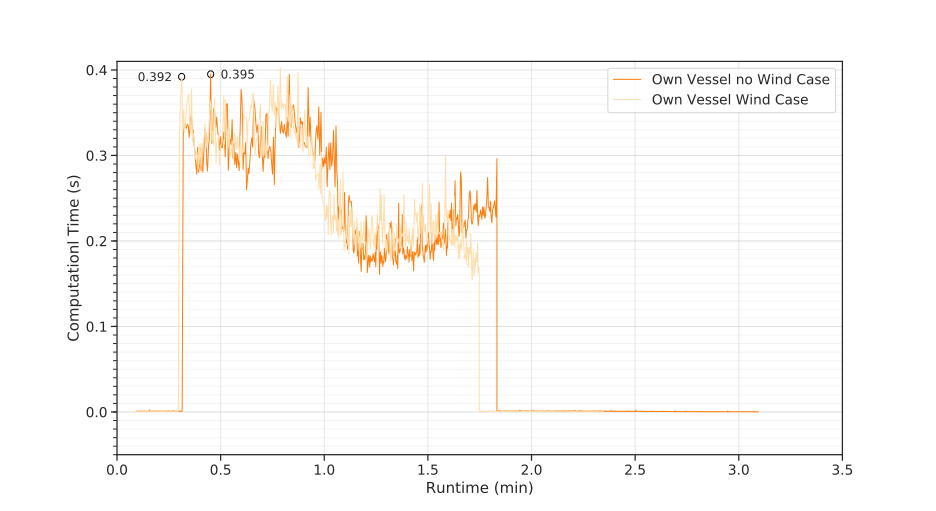
\includegraphics[width=\textwidth]{figs/Chap5/plot_cr_w_vs_wind_CT.png}
                \caption{Computation Time}
                \label{fig:plot_cr_w_vs_wind_CT}
            \end{subfigure}
        
        \caption{Head On Encounter Scenario with ATC, with and without wind. \ref{fig:plot_cr_w_vs_wo} and \ref{fig:plot_cr_w_vs_wo_CT}  description aqui. \ref{fig:plot_cr_w_vs_wind} and \ref{fig:plot_cr_w_vs_wind_CT} description aqui}
        \label{fig:plots_cr}
        \end{figure}
        
        %%%%%%%%%%%%%%%%%%%%%%%%%%%%%%%%%%%%%%
        %% Crossing Left w vs wo ATC. w vs wo Wind
        %%%%%%%%%%%%%%%%%%%%%%%%%%%%%%%%%%%%%%
        \begin{figure}[H]
        \centering
        
            \begin{subfigure}[b]{0.45\textwidth}
                \centering
                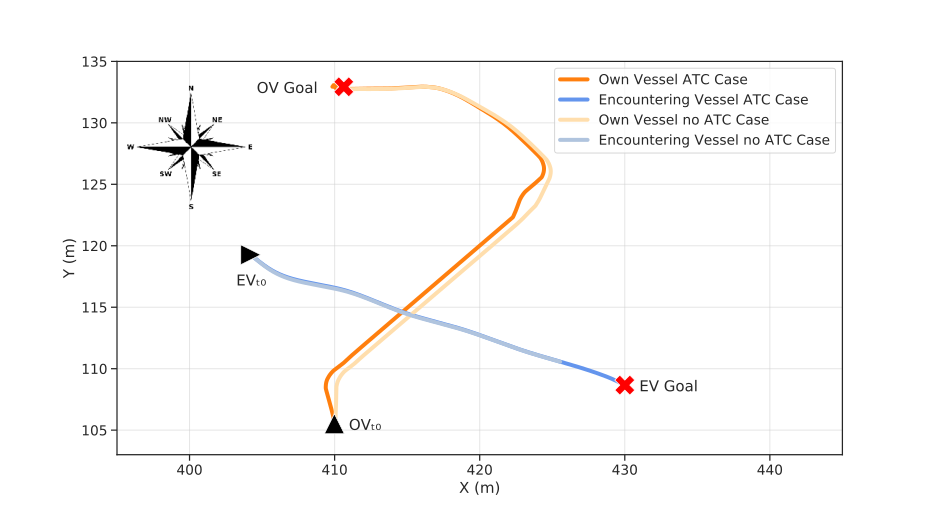
\includegraphics[width=\textwidth]{figs/Chap5/plot_cl_w_vs_wo.png}
                \caption{Route}
                \label{fig:plot_cl_w_vs_wo}
            \end{subfigure}
            \begin{subfigure}[b]{0.45\textwidth}
                \centering
                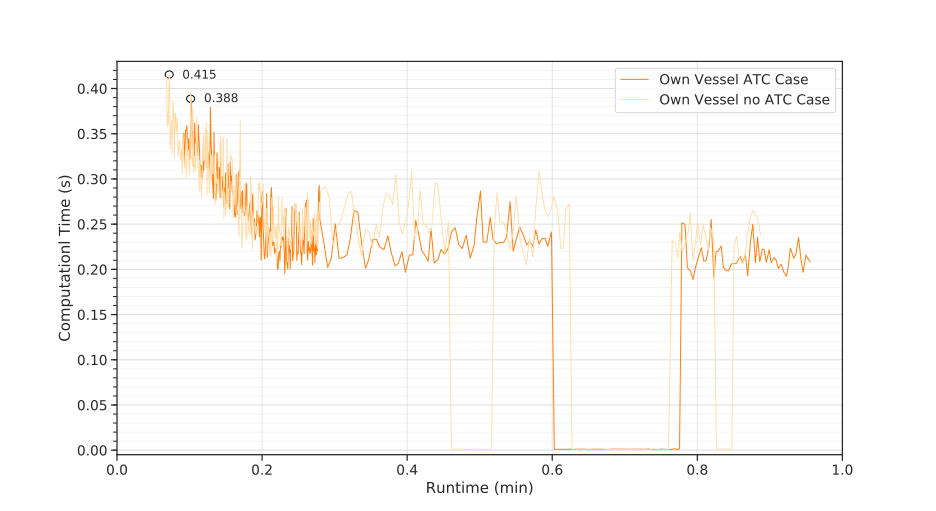
\includegraphics[width=\textwidth]{figs/Chap5/plot_cl_w_vs_wo_CT.png}
                \caption{Computation Time}
                \label{fig:plot_cl_w_vs_wo_CT}
            \end{subfigure}
            
            \begin{subfigure}[b]{0.45\textwidth}
                \centering
                \includegraphics[width=\textwidth]{figs/Chap5/plot_cl_w_vs_wind.png}
                \caption{Route}
                \label{fig:plot_cl_w_vs_wind}
            \end{subfigure}
            \begin{subfigure}[b]{0.45\textwidth}
                \centering
                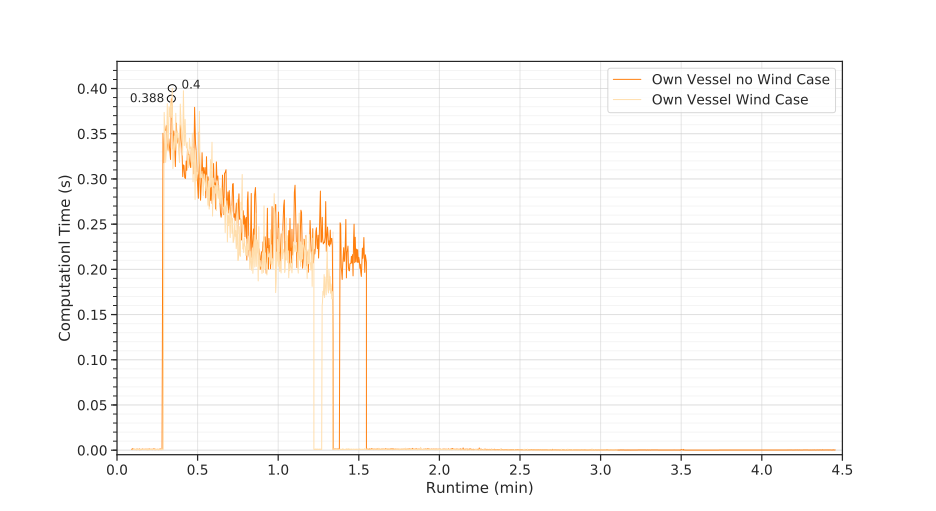
\includegraphics[width=\textwidth]{figs/Chap5/plot_cl_w_vs_wind_CT.png}
                \caption{Computation Time}
                \label{fig:plot_cl_w_vs_wind_CT}
            \end{subfigure}
        
        \caption{\ref{fig:plot_cl_w_vs_wo} and \ref{fig:plot_cl_w_vs_wo_CT}  description aqui. \ref{fig:plot_cl_w_vs_wind} and \ref{fig:plot_cl_w_vs_wind_CT} description aqui}
        \label{fig:plots_cl}
        \end{figure}
        
        %%%%%%%%%%%%%%%%%%%%%%%%%%%%%%%%%%%%%%
        %% Overtaking w vs wo ATC. w vs wo Wind
        %%%%%%%%%%%%%%%%%%%%%%%%%%%%%%%%%%%%%%
        \begin{figure}[H]
        \centering
        
            \begin{subfigure}[b]{0.45\textwidth}
                \centering
                \includegraphics[width=\textwidth]{figs/Chap5/plot_ov_w_vs_wo.png}
                \caption{Route}
                \label{fig:plot_ov_w_vs_wo}
            \end{subfigure}
            \begin{subfigure}[b]{0.45\textwidth}
                \centering
                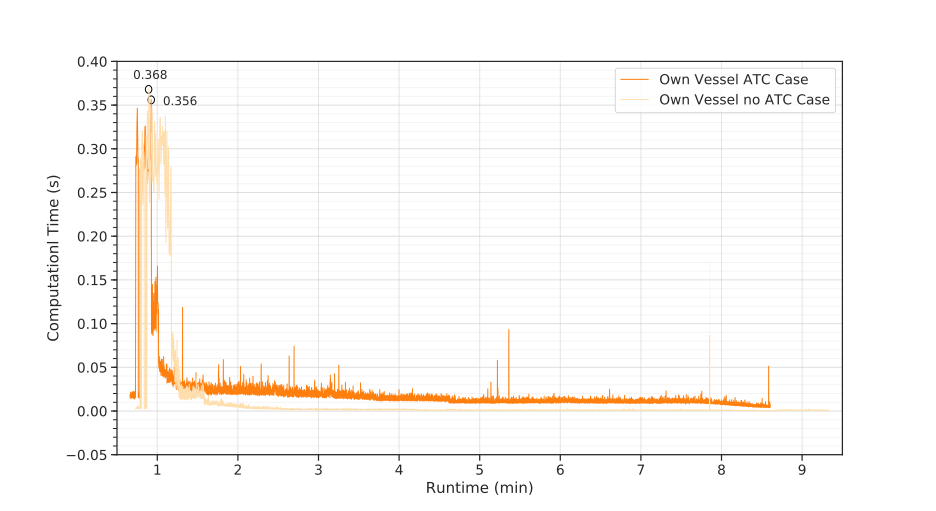
\includegraphics[width=\textwidth]{figs/Chap5/plot_ov_w_vs_wo_CT.png}
                \caption{Computation Time}
                \label{fig:plot_ov_w_vs_wo_CT}
            \end{subfigure}
            
            \begin{subfigure}[b]{0.45\textwidth}
                \centering
                \includegraphics[width=\textwidth]{figs/Chap5/plot_ov_w_vs_wind.png}
                \caption{Route}
                \label{fig:plot_ov_w_vs_wind}
            \end{subfigure}
            \begin{subfigure}[b]{0.45\textwidth}
                \centering
                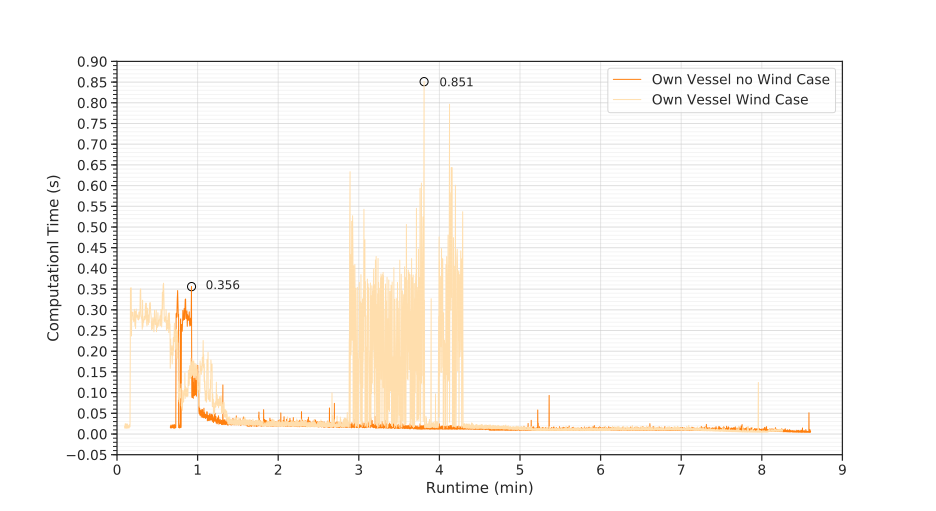
\includegraphics[width=\textwidth]{figs/Chap5/plot_ov_w_vs_wind_CT.png}
                \caption{Computation Time}
                \label{fig:plot_ov_w_vs_wind_CT}
            \end{subfigure}
        
        \caption{Head On Encounter Scenario with ATC, with and without wind. \ref{fig:plot_ov_w_vs_wo} and \ref{fig:plot_ov_w_vs_wo_CT}  description aqui. \ref{fig:plot_ov_w_vs_wind} and \ref{fig:plot_ov_w_vs_wind_CT} description aqui}
        \label{fig:plots_ov}
        \end{figure}

    
%AMA a diferenca entre avg e max eh enorme. explique bem o motivo disso. p um problema de tempo real, essa variacao nao eh muito interessante. 

\todo{cite authors on table caption}
\begin{table}
\caption{Based on \cite{} we made a quantitative evaluation of our planning system measuring computational cost and the minimum distance kept between the vessels during simulations.}
\centering
\begin{tabular}{|c|c|c|c|c|c|c|} 
\hline
\multirow{2}{*}{\textbf{Encounter} }                                                               & \multirow{2}{*}{\begin{tabular}[c]{@{}c@{}}\textbf{Scenario }\\\textbf{ Variation} \end{tabular}} & \multicolumn{3}{c|}{\begin{tabular}[c]{@{}c@{}}\textbf{Computational }\\\textbf{ Time (s)} \end{tabular}} & \multirow{2}{*}{\begin{tabular}[c]{@{}c@{}}\textbf{Successful }\\\textbf{ Avoidance} \end{tabular}} & \multirow{2}{*}{\begin{tabular}[c]{@{}c@{}}\textbf{Minimum }\\\textbf{ Distance (m)} \end{tabular}}  \\ 
\cline{3-5}
                                                                                                   &                                                                                                   & \textbf{Max.}  & \textbf{Average}  & \textbf{Std. Deviation}                                              &                                                                                                     &                                                                                                      \\ 
\hline
\multirow{3}{*}{\textbf{Head-On} }                                                                 & \textbf{No ATC}                                                                                   & 0.369          & 0.074             & 0.081                                                                & Yes                                                                                                 & 4.431                                                                                                \\ 
\cline{2-7}
                                                                                                   & \textbf{ATC}                                                                                      & 0.364          & 0.076             & 0.076                                                                & Yes                                                                                                 & 1.599                                                                                                \\ 
\cline{2-7}
                                                                                                   & \textbf{Wind}                                                                                     & 0.355          & 0.077             & 0.079                                                                & Yes                                                                                                 & 1.505                                                                                                \\ 
\hline
\multirow{3}{*}{\begin{tabular}[c]{@{}c@{}}\textbf{Crossing }\\\textbf{ from Right} \end{tabular}} & \textbf{No ATC}                                                                                   & 0.390          & 0.050             & 0.098                                                                & Yes                                                                                                 & 5.414                                                                                               \\ 
\cline{2-7}
                                                                                                   & \textbf{ATC}                                                                                      & 0.395          & 0.052             & 0.104                                                                & Yes                                                                                                 & 3.264                                                                                                \\ 
\cline{2-7}
                                                                                                   & \textbf{Wind}                                                                                     & 0.403          & 0.085             & 0.124                                                                & Yes                                                                                                 & 3.739                                                                                                \\ 
\hline
\multirow{3}{*}{\begin{tabular}[c]{@{}c@{}}\textbf{Crossing }\\\textbf{ from Left} \end{tabular}}  & \textbf{No ATC}                                                                                   &           &              &                                                                &                                                                                                &                                                                                                 \\ 
\cline{2-7}
                                                                                                   & \textbf{ATC}                                                                                      &               &                   &                                                                      &                                                                                                     &                                                                                                      \\ 
\cline{2-7}
                                                                                                   & \textbf{Wind}                                                                                     &                &                   &                                                                      &                                                                                                     &                                                                                                      \\ 
\hline
\multirow{3}{*}{\textbf{Overtaking} }                                                              & \textbf{No ATC}                                                                                   &   0.368             &  0.006                 &  0.030                                                                    &   Yes                                                                                                  &  3.325                                                                                                    \\ 
\cline{2-7}
                                                                                                   & \textbf{ATC}                                                                                      & 0.357          & 0.018             & 0.022                                                                & Yes                                                                                                 & 3.101                                                                                                \\ 
\cline{2-7}
                                                                                                   & \textbf{Wind}                                                                                     & 0.852          & 0.039             & 0.073                                                                & Yes                                                                                                 & 1.787                                                                                                \\
\hline
\end{tabular}
\label{tab:results}
\end{table}